\section{Conclusion et perspectives}

\begin{frame}{Conclusion}
  
  \textbf{\large L'édition collaborative temps réel est-elle possible sur le Web
    sans l'intervention d'un tiers et sans limites quant aux dimensions du
    système ? \YES{\cmark}}

  \vspace{1cm}

  Contributions :
  \begin{enumerate}
  \item %\textbf{taille des messages :}
    Fonction d'allocation d'identifiants polylogarithmique par rapport au nombre
    d'insertions dans la séquence; \vspace{0.2cm}
  \item %\textbf{nombre de messages :}
    Protocole d'échantillonnage adaptatif fournissant des vues logarithmiques
    par rapport à la taille du réseau supportant le processus de connexion des
    navigateurs Web.
  \end{enumerate}

\end{frame}


\begin{frame}{Conclusion}{Perspectives : compromis entre causalité et concurrence}
  
  Localement, \CRATE utilise toujours un vecteur de $N$ entiers où $N$ est le
  nombre de personnes ayant jamais participé à l'édition.
  
  \vspace{0.5cm}

  Remplacer ce vecteur de taille $N$ par un vecteur de taille $K$, $K\ll N$
  dépendant du taux de concurrence.

  \vspace{0.5cm}

  Intuition : sans concurrence, $K=1$ serait suffisant pour caractériser toutes
  les relations causales.

  \vspace{0.5cm}

  Cependant, une procédure est toujours nécessaire dans les cas ambigus.

\end{frame}


\begin{frame}{Conclusion}{Perspectives : O'Browser, Where Art Thou ?}

  \CRATE est un éditeur collaboratif décentralisé fonctionnant dans les
  navigateurs.

  \vspace{0.25cm}

  Quelles autres applications décentralisées est-il possible de développer ?

  \vspace{0.25cm}
  
  \begin{center}
    \begin{tikzpicture}[scale=0.8]

\newcommand\X{25pt}
\newcommand\Y{20pt}

\newcommand\LIGHTGRAY{gray!20}
\newcommand\MEDIUMGRAY{gray!40}

\tiny
%% communication
\draw[rounded corners=2mm, color=\MEDIUMGRAY, fill=white](0pt, 0pt)+(-4*\X,-\Y)rectangle+(4*\X,\Y);
\draw(4*\X, \Y)node[anchor=north east]{\textbf{communication}};

\draw[fill=white](-2*\X, -0.25*\Y)
node{dissémination}+(-0.85*\X,-0.5*\Y)rectangle+(0.85*\X,0.5*\Y);
\draw[fill=white, very thick, draw=darkblue]( 0*\X, 0.25*\Y)
node[align=center]{\DARKBLUE{appartenance}}+(-0.85*\X,-0.5*\Y)rectangle+(0.85*\X,0.5*\Y);
\draw[fill=white]( 2*\X, -0.25*\Y)
node{monodiffusion}+(-0.85*\X,-0.5*\Y)rectangle+(0.85*\X,0.5*\Y);

\draw[<-](-0.85*\X, 0.25*\Y)--(-1.15*\X, -0.25*\Y);
\draw[<-](0.85*\X, 0.25*\Y)--(1.15*\X, -0.25*\Y);

%% causality
\draw[rounded corners=2mm, color=\MEDIUMGRAY, fill=\LIGHTGRAY](0pt, -2*\Y)+(-4*\X,-\Y)rectangle+(4*\X,\Y);
\draw(4*\X, -\Y)node[anchor=north east]{\textbf{causalité}};

\draw[fill=\LIGHTGRAY](-2*\X, -2*\Y)
node[align=center]{détection\\[-1mm]des relations\\[-1mm]causales}
+(-1.0*\X,-0.6*\Y)rectangle+(1.0*\X,0.6*\Y);
\tiny
\draw[->, thick](-1.5*\X, -0.75*\Y) -- node[anchor=west]{reçoit}
(-1.5*\X, -1.4*\Y);
\draw[<-, thick](-2.5*\X, -0.75*\Y) -- node[anchor=east]{envoie}
(-2.5*\X, -1.4*\Y);
\tiny
\draw[<->]( 2*\X, -0.75*\Y)--( 1*\X, -2.5*\Y);

%% sequence structure
\draw[rounded corners=2mm, color=\MEDIUMGRAY, fill=white](0pt, -4*\Y)+(-4*\X,-\Y)rectangle+(4*\X,\Y);
\draw(4*\X, -3*\Y)node[anchor=north east, align=right]
{\textbf{structure}\\\textbf{pour}\\\textbf{séquences}};

\draw[fill=white, shading=axis,top color=\LIGHTGRAY, bottom color=white, shading angle=0](1*\X, -3*\Y)
node{anti-entropie}+(-0.95*\X,-0.5*\Y) rectangle +(0.95 *\X, 0.5*\Y);
\draw[fill=white, very thick, draw=darkblue](-2*\X, -4*\Y)
node{\DARKBLUE{réplique}}+(-0.75*\X,-0.5*\Y) rectangle +(0.75 *\X, 0.5*\Y);

\draw[->] (0.05*\X, -2.75*\Y)--(-1*\X,-2*\Y);
\draw[->] (0.05*\X, -3.25*\Y)--(-1.25*\X,-4*\Y);
\tiny
\draw[<-, thick] (-1.5*\X, -3.5*\Y)--node[anchor=west]{délivre}(-1.5*\X, -2.6*\Y);
\draw[->, thick] (-2.5*\X, -3.5*\Y)--node[anchor=east]{décore}(-2.5*\X, -2.6*\Y);
\tiny
%% gui
\draw[rounded corners=2mm, color=\MEDIUMGRAY, fill=\LIGHTGRAY](0pt, -6*\Y)+(-4*\X,-\Y)rectangle+(4*\X,\Y);
\draw(4*\X, -5*\Y)node[anchor=north east, align=right]
{\textbf{interface}\\\textbf{utilisateur}};
\draw[fill=\LIGHTGRAY](0pt,-6*\Y)
node{éditeur web}+(-0.85*\X,-0.5*\Y) rectangle +(0.85 *\X, 0.5*\Y);

%%\draw[<->] (-2*\X, -4.5*\Y) -- (0*\X, -5.5*\Y);
\tiny
\draw[->, thick] (-1.80*\X, -4.5*\Y)--node[anchor=west]{notifie}(-0.85*\X, -5.75*\Y);
\draw[<-, thick] (-2.20*\X, -4.5*\Y)--node[anchor=east]{met à jour}(-0.85*\X, -6.25*\Y);
\tiny
\end{tikzpicture}
  \end{center}

\end{frame}


\begin{frame}
  
  \begin{center}
    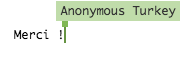
\includegraphics[width=0.55\textwidth]{img/thanks.png}
  \end{center}

\end{frame}